%!TEX root = ../thesis.tex
%*******************************************************************************
%*********************************** First Chapter *****************************
%*******************************************************************************

\chapter{Introduction} %Title of the First Chapter

\ifpdf
    \graphicspath{{Chapter1/Figs/Raster/}{Chapter1/Figs/PDF/}{Chapter1/Figs/}}
\else
    \graphicspath{{Chapter1/Figs/Vector/}{Chapter1/Figs/}}
\fi

What physical driving factors led to the proliferation of multicellular life?
Across all eukaryotic lineages, phylogenetic evidence suggests that multicellularity evolved independently several times \citep{king2004}.
Within just the volvocine algae, a common model family for studying the origins of multicellularity, it is believed that the transition to multicellularity and cooperation of distinct differentiated cells has repeatedly emerged independently \citep{herron2008}.
Given the overwhelming success of multicellular life in the biosphere, we are led to hypothesize that common physical advantages promoted life to cooperate, differentiate, and delegate the responsibility of ensuring fitness for the sake of proliferation \citep{grosberg2007}.

This question has led to flourishing recent interest in evolutionarily basal model eukaryotes, especially choanoflagellates, volvocine green algae, and sponges.
Both the biological and physical properties of these groups make them favorable \citep{goldstein2015}: choanoflagellates have long been regarded as a close relative to the animal kingdom owing to their similarity to choanocytes in sponges \citep{james1871}, and the volvocine algae span a range of cell numbers per individual \citep{kirk2005}.
These organisms and their colonies are also large enough that they operate at high P\'eclet number ($Pe \sim 10^2$), the ratio between advective and diffusive transport, meaning that advection must contribute substantially to deriving food \citep{solari2006}. 
Consequently, these organisms must facilitate their food collection, unlike bacteria which rely on diffusion for nutrient transport \citep{berg1977}.

%********************************** %First Section  **************************************
\section{Multicellularity} %Section - 1.1 

% \textbf{Thesis statement: studying evolutionarily basal organisms lets us study the simple ways that nature exploits geometry in living systems without higher order functional complications.}

\begin{comment}

\nomenclature[z-cif]{$CIF$}{Cauchy's Integral Formula}                                % first letter Z is for Acronyms 
\nomenclature[a-F]{$F$}{complex function}                                                   % first letter A is for Roman symbols
\nomenclature[g-p]{$\pi$}{ $\simeq 3.14\ldots$}                                             % first letter G is for Greek Symbols
\nomenclature[g-i]{$\iota$}{unit imaginary number $\sqrt{-1}$}                      % first letter G is for Greek Symbols
\nomenclature[g-g]{$\gamma$}{a simply closed curve on a complex plane}  % first letter G is for Greek Symbols
\nomenclature[x-i]{$\oint_\gamma$}{integration around a curve $\gamma$} % first letter X is for Other Symbols
\nomenclature[r-j]{$j$}{superscript index}                                                       % first letter R is for superscripts
\nomenclature[s-0]{$0$}{subscript index}                                                        % first letter S is for subscripts
\end{comment}

\nomenclature[a-pe]{$Pe$}{P\'eclet number, the ratio between advective and diffusive transport in a fluid with specified flow velocity and length scale}
\nomenclature[z-ECM]{ECM}{Extracellular matrix}

\subsection{Origins of multicellularity}

% prokaryotic multicellularity
Before discussing eukaryotic multicellularity, I would be remiss in neglecting prokaryotic multicellularity \citep{shapiro1988}. 
Beyond the notorious biofilm formation, cyanobacteria (e.g. \textit{Anabaena}) form chains of cells as filaments and some sporulating bacteria (e.g. Myxobacteria, \textit{Steptomyces}) form fruiting bodies \citep{claessen2014}.
These multicellular aggregates demonstrate complex population dynamics and emergent collective behavior from basic interactions \citep{lopez2010,welch2001,zhang2012}.
Biofilms and filaments have phenotypically diverse and even differentiated regions that contribute to antibiotic resistance \citep{stewart2008} or enable photosynthesis \citep{flores2010}
This differentiation can parallel germ-soma differentiation in eukaryotes by sacrificing individual division for colony persistence \citep{lewis2010,wilcox1973}.
Moreover, the extracellular matrix (ECM) of biofilms allows bacteria to exploit a tradeoff between environmental protection and growth by slowing diffusion from the exterior \citep{mah2001,rittmann1980}.
The rest of this work centres around eukaryotic multicellularity, but it is valuable to keep in mind that several multicellular organisms have bacterial parallels.

The benefit of multicellularity for individual cells is not immediate.
\citet{michod2003} argues that a key transition in the development of multicellularity is the transition away from selecting for single cell fitness to multicellular fitness. 
Indeed, while several pathways for multicellularity have been proposed, they share the idea that emergent group benefits through cooperation sufficiently outweigh individual sacrifice \citep{michod2001}.

Multicellularity requires that resources are shared, and \textit{cheat cells} which exploit this cooperation arise.
Several have argued that exploitation and internal conflict may have facilitated evolution and differentation that contributes to individuality of the whole organism \citep{michod2001,rainey2010,hammerschmidt2014,grosberg2007}.
Aggregative multicellularity is believed to be uncommon because the genetic variation across solitary cells makes it easy for cheat cells to arise; the required similarity in these organisms makes division of labor limited \citep{brunet2017}.
On the other hand, an altruistic strategy allows cells to cooperate and help each other, increasing the success of the colony more than the sum of the individual cells \citep{michod2006,gulli2019}.

\subsection{Benefits} \label{subsec:benefits}
\paragraph*{Size}
% size
A major competing argument for the origin of multicellularity centers around physical size. 
\citet{bonner1998} argues that size enables the advantages conferred by multicellularity, and scale itself comprises a spectrum of niches available for exploitation.
An immediate consequence of an increase in size is the ability to avoid predation via phagocytosis.
\citet{stanley1973} argues that the emergence of heterotrophs, or organisms that derive energy by consuming others, led to rapid diversification and the rise of multicellularity through intense selective pressure. 
\citet{boraas1998} demonstrated in a laboratory culture that stable multicellularity emerged in the green alga \textit{Chlorella vulgaris} when exposed to predators.
Eight-cell colonies were observed to predominate, indicating that multicellularity emerged to balance colony survival as well as individual demands of each cell.

% division of labour
\paragraph*{Division of labour} Differentiation of isolated cells by time-varying gene expression or generational life stages enables the division of labour in time \citep{grosberg2007,brunet2017}.
Multicellularity, on the other hand, makes it possible for several cooperating cells to distribute the responsibility of survival and propagation in space.
In eukaryotes, differentation into either germ or soma cells for the sake of reproduction is a common feature of multicellular organisms \citep{cheng2020}. 
Spatial constraints to cellular organisation generally produces a sparse interaction network between cells, which is thought to favour division of labour for reproduction \citep{yanni2020}.

Best studied in the primitive models of multicellularity is germ-soma differentiation in the volvocine green algae, especially the genus \textit{Volvox}.
The species in the volvocines span several orders of magnitude in cell number and size connected by an extracellular matrix and intracellular bridges \citep{larson1992,kirk2005}.
\textit{Volvox} individuals form hollow, spherical embryos that characteristically invert by forming a hole at one end \citep{viamontes1977,kirk2001}.
The benefit of differentiation is thought to scale with colony size, where reproductive costs become cumbersome as the organism becomes larger \citep{solari2006a,solari2013}.

Division of labour has been observed to emerge even when selecting for organism size.
Baker's yeast \textit{Saccharomyces cerevisiae} was found to develop multicellularity through repeated cell division (as opposed to aggregation) when selecting for the settling rate out of liquid culture.
Despite being chosen for size, these \textit{snowflake} clusters had a minority of cells differentiated to perform apoptosis, causing the cluster to fragment and divide the cluster into several more \citep{ratcliff2012}. 

% * Attaching supports flows
\paragraph*{Generating flows} With size increasing the P\'eclet number for an organism ($Pe = Lu/D$, where $L$ is the length scale, $u$ is flow velocity, and $D$ is diffusion coefficient), multicellular organisms benefit more from advective nutrient transport as they become larger. 
The volvocine algae increase the proportion of advective flux as they increase in size by generating a thin boundary layer in solute concentration, in turn facilitating long-range nutrient transport \citep{short2006}.

The advantages of multicellularity for choanoflagellate flows are yet unclear. 
\citet{kirkegaard2016} modeled that the best flows through a collar of microvilli are generated when cells swim independently, aligning with the idea that unicellular swimming is optimal feeding \citep{michelin2011}. 
Rosette choanoflagellate colonies are even worse at generating flows through collars, as their flagella all point in different directions. 

For the colony geometries studied in this work, however, we may compare to sponge choanocyte chambers and the substantial flows they are capable of producing. 
Sponges drive flow using choanocytes, which are morphologically and functionally similar to choanoflagellates despite being animal cells \citep{larsen1994,carr2008}.
By organising into spherical chambers, sponges are able to efficiently generate flows and chain together pumps to drive macroscopic flow \citep{asadzadeh2019}.
Deriving from the first animals, sponges bring the evolutionary conclusions from these models for basic multicellularity closer to increasingly complex animals \citep{nielsen2008}.

%********************************** %Second Section  *************************************
\section{Choanoflagellates} \label{sec:choano} %Section - 1.2 

Choanoflagellates are aquatic heterotrophs that feed in their motile stage by driving flows through a collar of microvilli using a single apical flagellum \citep{karpov1998} (\cref{subfig:morphology}).
Choanoflagellates are considered the genetically closest group to metazoans \citep{carr2008}, though the association between choanoflagellates and animals predates studies using molecular phylogeny.
\citet{james1871} first compared choanoflagellate morphology with the choanocytes in sponge choanocyte chamber. 
Morphological similarities between choanocytes and protists led to the belief that the two emerged from a common ancestor \citep{saedeleer1930,tuzet1963}.

Sponge choanocytes and choanoflagellate morphology bear substantial resemblence to each other in that both collars and apical flagella.
However, choanoflagellate cells always have collar filaments, while choanocytes develop them through differentiation \citep{mah2014}.
Choanoflagellate glycocalyx tends to surround the cell body, while sponges use it to form a web with the collar microvilli \citep{leadbeater2008}.

Choanoflagellates are increasingly studied as a model for understanding how multicellular animal life emerged. 
Much of the recent work on choanoflagellates has been done with \textit{Salpingoeca rosetta}, a model for the development of multicellularity for its propensity to form multicellular rosettes bound by an extracellular matrix (ECM).
Based on \textit{S. rosetta} studies, our understanding of choanoflagellate colony formation is that single cells initiate colonies by cell division, rather than aggregation \citep{fairclough2010}.
Additionally, choanoflagellate colony morphology appears to be dictated by the ECM material properties, producing a variety of structures attached at cell bodies \citep{larson2020}.

The reasons for colony formation (i.e. multicellularity) in choanoflagellates are unclear, especially from a flow perspective (\cref{subsec:benefits}). 
Evolutionary causes of colony formation are obscured further by strong recent evidence that rosette formation in \textit{S. rosetta} is induced by chemical cues from bacteria \citep{alegado2012,woznica2016}.

%********************************** % Third Section  *************************************
\section{\textit{Choanoeca flexa}}  %Section - 1.3 

% intro`
\citet{brunet2019} describe a newly discovered choanoflagellate, \textit{Choanoeca flexa}, which lives and feeds in aquatic environments (\cref{fig:cflexa}). 
Here, I describe the relevant properties and characteristics of these cells and their colonies for modeling its structure and behavior. 
All descriptions of \textit{C. flexa} proceed from \citet{brunet2019} and private communications with the authors.

\begin{figure}[htbp]
	\centering
	\begin{subfigure}[b]{0.5\textwidth}
		\centering
		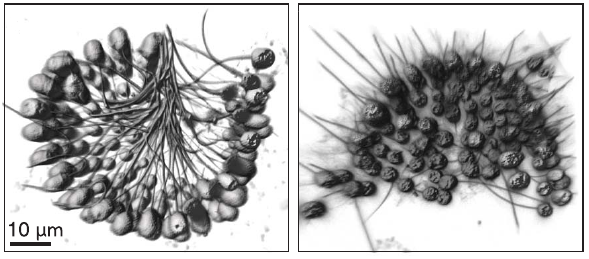
\includegraphics[width=\textwidth]{cflexa.png}
		\caption{}
		\label{subfig:cflexa}
	\end{subfigure}
	\begin{subfigure}[b]{0.18\textwidth}
		\centering
		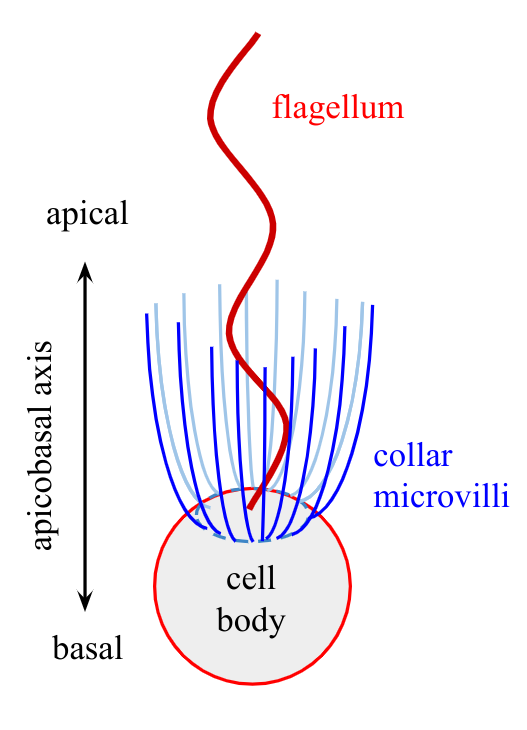
\includegraphics[width=\textwidth]{morphology.png}
		\caption{}
		\label{subfig:morphology}
	\end{subfigure}
	\begin{subfigure}[b]{0.3\textwidth}
		\centering
		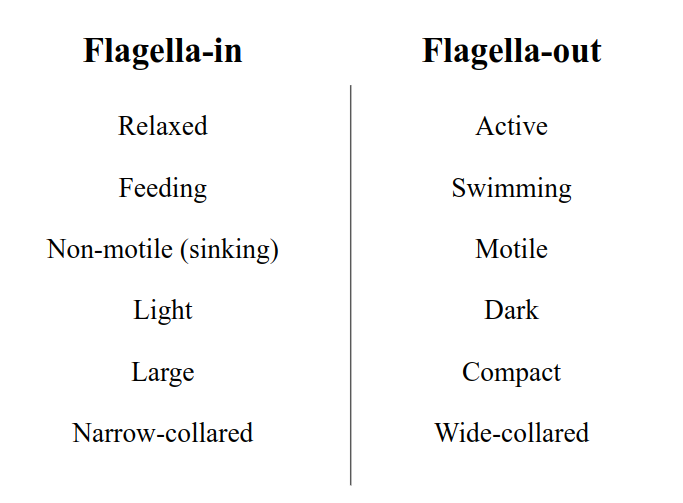
\includegraphics[width=\textwidth]{table.png}
		\caption{}
		\label{subfig:table}
	\end{subfigure}
	\begin{subfigure}[b]{0.56\textwidth}
		\centering
		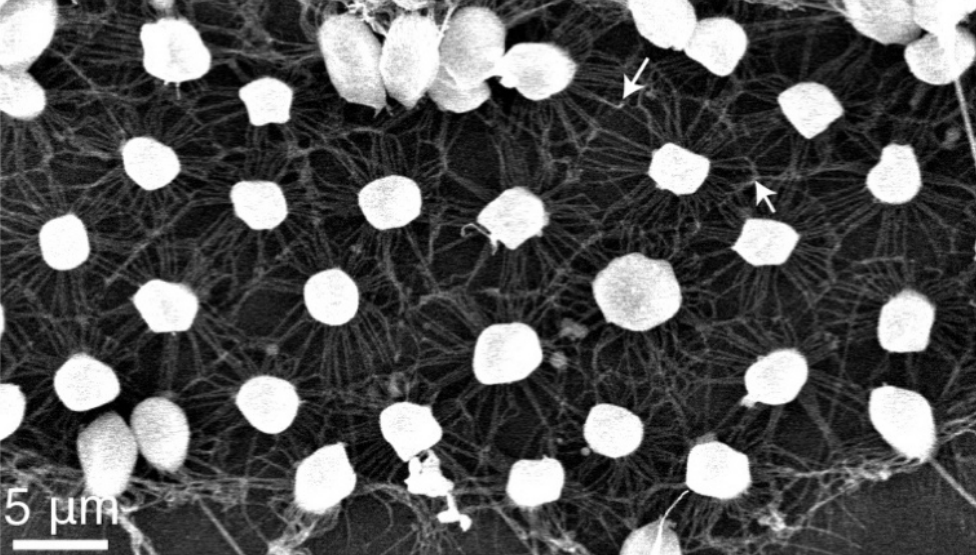
\includegraphics[width=\textwidth]{contact1.png}
		\caption{}
		\label{subfig:contact1}
	\end{subfigure}
	\begin{subfigure}[b]{0.43\textwidth}
		\centering
		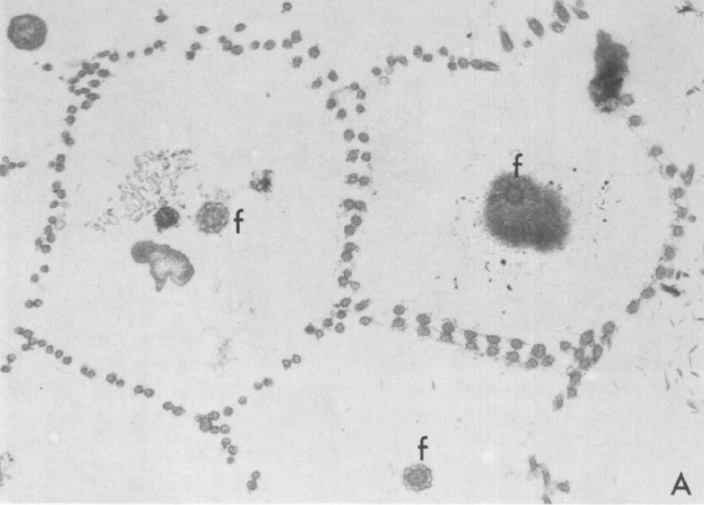
\includegraphics[width=\textwidth]{contact2.png}
		\caption{}
		\label{subfig:contact2}
	\end{subfigure}
	\caption[Overview of \textit{C. flexa} colonies of collared choanoflagellate cells]{Overview of \textit{C. flexa} colonies of collared choanoflagellate cells. (\ref{subfig:cflexa}) Images of the two conformations observed, flagella-in and flagella out. (\ref{subfig:morphology}) The morphology of a single \textit{C. flexa} colonial cell. (\ref{subfig:table}) Summary of the two states of \textit{C. flexa} colonies. The transition from flagella-in to flagella-out is induced naturally by darkness, and the reverse transition is induced by the reintroduction of light \citep{brunet2019}. (\ref{subfig:contact1}) Scanning electron micrograph in the tangential plane of a \textit{C. flexa} sheet. Arrows indicate collar-collar contacts. (\ref{subfig:contact2}) Transmission electron micrograph of collar interactions between neighboring cells in a \textit{C. perplexa} colony. f: flagella. From \citet{leadbeater1983} with permission. \cref{subfig:cflexa,subfig:contact1} from \citet{brunet2019}. Reprinted with permission from AAAS.}
	\label{fig:cflexa}
\end{figure} 

% general description
\textit{C. flexa} is an aquatic colonial choanoflagellate that forms sheets on the order of $\SI{100}{\micro\meter}$ in diameter (\cref{fig:cflexa}).
Each cell in a colony consists of a cell body ($\sim \SI{4}{\micro\meter}$), microvillar collar ($\sim\SI{10}{\micro\meter}$ length), and apical flagellum at the collar centre (\cref{subfig:morphology}).
All observed sheets have had flagella facing in the same direction, giving the sheet two distinct sides.
Cells attach to each other through their collar microvilli, and in contrast to a colonial flagellate like \textit{S. rosetta}, there is no evidence for an extracellular matrix holding cells together in \textit{Choanoeca} \citep{leadbeater1983,brunet2019}.
Collar microvilli are distinct and colony cells demonstrated no intercellular cytoplasmic bridges or ECM (contrast with \textit{i.e. Volvox}), with cells detaching from each other upon treatment with calcium \citep{thibaut}.
\mynote{double check that it was calcium!}
By comparison with division in \textit{C. perplexa}, colony cells are expected to undergo cell division with temporary incomplete replication, where the pair of daughter cells is attached by some shared collar microvilli (\cref{fig:division}).
Colonies are believed to occasionally fragment to separate completely and multiply \citep{leadbeater1983}.

% thecate and division
\textit{C. flexa} also exhibits a sedentary, unicellular form that adheres to surfaces via a stalk (\textit{theca}) without a flagellum, as in \textit{C. perplexa}.
Our understanding of cell division in \textit{Choanoeca} emerges from the thecate form, which leaves one thecate daughter cell and another motile, flagellated cell.
Division begins with the generation of a flagellum by the thecate cell and proceed with protoplasm division with incomplete separation at collar microvilli (\cref{fig:division}) \citep{ellis1930,leadbeater1977}.
The remainder of this work concerns the colonial form of \textit{C. flexa} rather than the thecate or unicellular motile forms.
While we do not have observations on cell replication in the colonial phase, \textit{S. rosetta} gives a suggestion that colonial choanoflagellates do not coordinate their cell division \citep{fairclough2010}.

\begin{figure}[htbp]
	\centering
	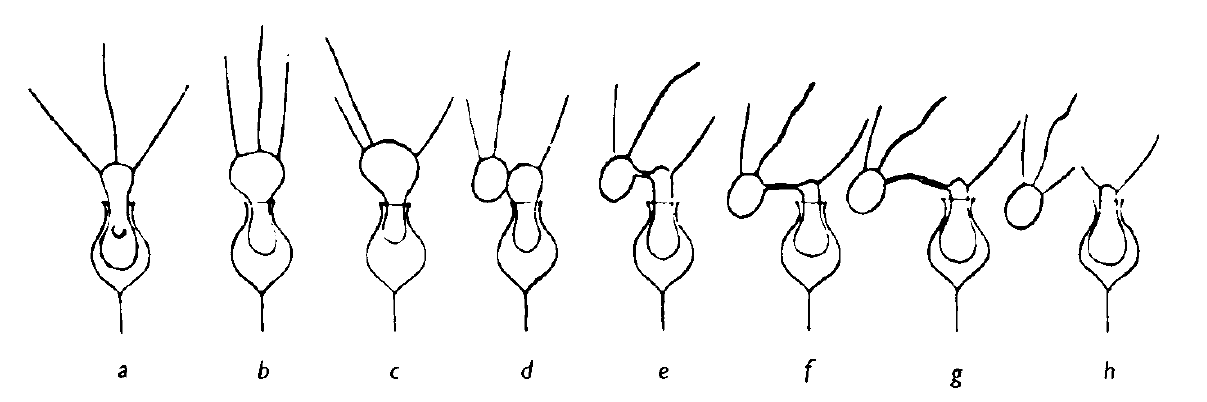
\includegraphics[width=\textwidth]{division.png}
	\caption[Illustrations of stages of division in the sessile form of \textit{C. perplexa}]{Illustrations of stages of division in the sessile form of \textit{C. perplexa}. Reproduced from \citet{leadbeater1977} based on \citet{ellis1930} with permission from Cambridge University Press.}
	\label{fig:division}
\end{figure}

% While choanoflagellate colonies typically orient their flagella to point away from the colony centre, sheets of \textit{Choanoeca} in their rest state point flagella inward. \mynote{cite this! \citet{brunet2019} uses a leadbeater textbook}

\subsection{Sheet inversion}

% inversion introduction
\textit{Choanoeca} has recently sparked renewed interest as a result of the characterisation of rapid light-regulated inversion in colonies, which causes cell sheets to change orientation from pointing flagella-in to flagella-out \citep{brunet2019}.
The inversion is understood to result from contraction of an actomyosin ring at the apical end of colony cells, which results in collar microvilli flaring out. 
This result is consistent with a description of contraction at the cell apex with changes in collar angle for \textit{C. perplexa} cells \citep{leadbeater1977}.
Sheet inversion takes $\sim\SI{10}{\second}$.
Notably, deviations in \textit{C. perplexa} collar angle (between $10^\circ-90^\circ$ from the apicobasal axis) were described in \citet{ellis1930}, and \citet{leadbeater1983} described colonies now understood to be \textit{C. perplexa} undergoing inversion. 
\footnote{The latter attributes inversion to a reversal of flagellum rotation, though this explanation is unlikely given the more recent evidence for \textit{C. flexa} \citep{brunet2019}.}
Collar stiffness and the intrinsic curvature in collars facilitates a clear preference in sheet curvature. 
Collars in thecate cells have been described as flaccid \citep{leadbeater1977}, suggesting that an increase in collar stiffness is essential to the transition to colony-forming cells. 

% describing two states
\citet{brunet2019} identified several factors that contribute or prohibit sheet inversion. 
It is believed that, in their natural environment, sheet inversion from flagella-in to flagella-out is triggered by darkness. 
In the inverted (flagella-out) state that occurs in darkness, individual cells demonstrated contraction of an apical actomyosin ring.
The contraction results in collar microvilli flaring out: relative to the apicobasal axis measured at the base of the flagellum, the median collar microvillus angle moved out from $\sim35^\circ$ to $\sim50^\circ$.
This increase in angle is largely the result of collar microvilli straightening out: in light, single colony-cells' collars curve to align with the apicobasal axis after emerging from the apical ends of cells.
\mynote{add figure of individual cells}
Cell sheet area decreases significantly since cell bodies are in contact in the inverted state \citep{thibaut}.
These properties are summarised in \cref{subfig:table}.

% what does inversion achieve?
The transition to the flagella-out state results in a significant increase in swimming speed \citep{brunet2019}. 
In contrast, flagella-in sheets are non-motile to the extent that they typically sink. 
The lack of mobility is compensated by an increase in cells phagocytosis by several times: flagella-in sheets are substantially more effective at driving flow towards the collars, where individual cells feed.
Increased motility in the dark-induced state and accumulation in regions with light facilitates a primitive form of phototaxis.
\mynote{why does swimming not directly translate to feeding as in lauga2011 paper?}

% dynamics
Sheet inversion is rapid and reversible, allowing colonies the flexibility to convert when given suitable environmental cues.
\mynote{discuss how larger sheets are harder to invert}


% Coordinated geometric changes in multicellular organisms are frequent, though they are typically achieved with several differentiated cell types or molecular signalling cascades \citep{todo}. 

% \section{Motivation and objective}
% 
% As in the other basal model organisms used to probe the evolution of multicellularity, \textit{C. flexa} offers a context to study the earliest driving factors towards multicellular shape change through cooperative individual action. 
% In addition to sharing similar geometry with sponge choanocyte chambers and directly informing structural modeling there \citep{asadzadeh2019}, \textit{C. flexa} captures the close relationship between geometry and flow in biological settings. 
% The suspected functionality of its inversion gives a potential evolutionary reason for colony formation in a choanoflagellate.

\section{Thesis overview}

\textit{C. flexa} provides an opportunity to study geometric changes through a simple, uncoordinated mechanism in an evolutionarily basal context. 
In this thesis, I present several approaches for modeling \textit{C. flexa} colony sheets from a mechanics perspective. 
I discuss relevant models from continuous mechanics and find that the simultaneous stretching and compression in several collar microvilli must be taken into account to appropriately model shape and dynamics. 
I review shape equations derived from variation of surface energies defined in terms of curvatures and derive an energy function for a continuous description of \textit{C. flexa} sheets. 

Due to the complexity of the continuous model, I develop a more tractable discrete model based on lessons from the continuous description. 
Collar microvilli are simplified from filaments to straight elastic rods, which permits a simple energy function to be defined in terms quadratic potentials on cell-collar distances and angles defined by connecting cells and collars.
The model consists of two parameters: equilibrium angles $\phi_0$ (preferred angle from the collar base to the apicobasal axis) and $\psi_0$ (preferred collar-collar contact angle). 
I take the gradient of the energy with respect to cell and collar coordinate vectors as well as the apicobasal axis vectors of all cells to solve the forces acting on all free variables in the system.
I numerically intergrate the forces on all spatial coordinates and torques on cell axes to study dynamics of cell sheets and study their mechanical equilibria.

My discrete model for \textit{C. flexa} colonies successfully models inversion in small sheets consisting of few cells. 
In larger sheets, conformational changes are hindered by rings of cells which cannot undergo the requisite stretching or compression required for inversion or folding. 
% For sheets with too many cells at the boundary, the inability to compress results in buckling at the edges. 
When sheets are already curved with flagella pointing in or out, the inability to sufficiently stretch at the boundary prevents sheets from inverting and causes the cells on the sheet interior to experience substantial stress.
By framing my discrete model of \textit{C. flexa} using graph theory, I identify that the topology of the cell-cell connection lattice determines a sheet's ability to bend without buckling or overstretching.
This finding and my structural results compare well with the understanding of geometric effects of topological defects in crystal lattices.

The model I present makes it possible to identify regions where equilibrium angles $\phi_0$ and $\psi_0$ give minimal energy structures in the flagella-in and -out conformations.
For values that facilitate a flagella-out structure, the flagella-out structure is lower in energy than the flagella-in structure when sheet size prevents inversion as expected.
I argue that the greater amount of time required for larger sheets to invert is the result of a larger energetic barrier or smaller net internal forces, rather than greater hydrodynamic damping through drag. 
This effect from topological constraints at the sheet boundary explains the rapid contraction and slow inversion observed in large sheets in \citep{brunet2019}.
My model supports the hypothesis that \textit{C. flexa} sheets are able to invert as a result of extreme stretching at sheet boundaries or topological changes through collar-collar linkages temporarily breaking.
